\chapter{\texorpdfstring{\MakeUppercase{Summary and Future Outlook}}{Summary and Future Outlook}} \label{chap:summary}

\section{Summary}

This dissertation has followed one common thread across six years of research: modeling astrophysical turbulence across scales by connecting observable tracers, numerical simulations, and machine-learning diagnostics.
Astrophysical turbulence regulates the transport of matter and energy, from galaxy-scale driving down to dissipation scales only a few kilometers across.
Between these extremes in spatial scale lie galactic accretion flows onto active galactic nuclei (AGNs), star formation in molecular clouds, and extreme electromagnetic events near accreting supermassive black holes (SMBHs).
Across these environments, a common difficulty in understanding turbulence is that it is rarely observed directly or numerically modeled without some form of compromise.
Instead, turbulence is often inferred from imperfect tracers and simulations that resolve only part of the dynamical range.
The chapters in this dissertation address these difficulties by developing diagnostic tools tailored to three representative turbulence regimes.

\subsection{Using young stars to study interstellar turbulence}

In Chapter~\ref{chap:stars}, I presented a new method to measure the level of turbulence in star-forming regions with young stars.
Historically, turbulence in Milky Way molecular clouds had been measured through line-width observations of gas tracers, including \halpha, \ion{H}{1}, CO, and HCN\@.
These measurements were precise in the plane-of-the-sky position (only limited by the telescope's beam resolution) and line-of-sight (LOS) velocity (inferred from the shift in wavelength of the tracer), but they provided no information about the other three kinematic dimensions.
Gas-based turbulence measurements were, therefore, severely restricted by projection effects, and conclusions drawn through this method had to contend with a multitude of uncertainties.
Using young stars as turbulence tracers significantly reduces these uncertainties.

In \citet{ha_measuring_2021}, we hypothesized that, since young stars are born out of turbulent molecular clouds, the stars would inherit these turbulent statistics at the region scale.
We obtained six-dimensional (6D) kinematics from the Gaia and APOGEE-2 surveys of 1439 stars in the Orion Molecular Cloud Complex and computed the first-order velocity structure function (VSF) for each subgroup in the region.
We found that in regions where star formation is sparse, the VSFs resemble a Kolmogorov turbulent scaling.
This finding supported our hypothesis and indicated that young stars could indeed serve as a tracer of turbulence in certain conditions.
We also found, on the other hand, that the VSFs from dense star clusters (the Orion Nebula Cluster) were less useful, exhibiting no such power-law scaling.
We explained this lack of turbulent scaling as a direct consequence of dynamical relaxation---the motion of newly formed stars is quickly perturbed by nearby stars, changing their trajectories and erasing the memory of turbulence shortly after formation.
We also commented on another limitation of using stars as a turbulent tracer, namely that stars naturally lose their memory of turbulence through drifting over the crossing time of the region.
These limitations restrict the types of regions in which our proposed method can meaningfully provide turbulence constraints in addition to gas tracers.

In \citet{ha_turbulence_2022}, we formalized our proposed method by extending our coverage to four star-forming regions: Orion, Ophiuchus, Perseus, and Taurus.
We also obtained \halpha\ and CO data for direct comparison between stellar and gas tracers.
In agreement with the previous work, we found a universal scaling of turbulence in all four regions, indicating that young stars are effective tracers of turbulence in star-forming regions and that the turbulent cascade is likely controlled by a Galactic-scale driver.
We also identified a characteristic ``bump'' in the VSF of two regions, Orion and Ophiuchus, which we mapped to analytically confirmed supernovae (SNe) that took place several million years ago.
These SNe injected a large amount of kinetic energy into the two systems, raising the level of turbulence, which steepened the slope of the VSFs.
These events also carried over to the \halpha\ VSFs, where the amplitudes of the VSFs in Orion and Ophiuchus were significantly higher than the VSF of stars.
On the other hand, the VSFs of \halpha\ and stars are roughly consistent in the other two regions.
We concluded that SNe inject energy unevenly into different phases of gas, efficiently driving low-density, volume-filling ionized gas such as \halpha, while affecting the high-density, clumpy molecular gas that forms stars differently.
These two papers suggested a complex picture of the Milky Way interstellar medium (ISM), where turbulence can be driven at different scales and inject energy unevenly into different phases.

Since these works were published, the method has been adopted and extended in several studies of nearby star-forming regions and the molecular ISM\@.
\citet{krolikowski_gaia_2021} studied the Taurus-Auriga region with Gaia EDR3, and showed that the stellar velocity structure retains an initial turbulent spectrum similar to Larson's law before being modified by the dynamical evolution of the association.
\citet{zhou_kinematics_2022} applied the same idea to 150 young stellar object (YSO) associations, using their motions to probe molecular cloud turbulence, velocity dispersion--size scaling, isotropy, and the Galactocentric dependence of turbulent energy dissipation.
Then, \citet{zhou_gas_2024} used the same YSO associations as cloud tracers to compare young-star distributions against CO and dust, and connect feedback-driven gas removal to the velocity dispersion--size relation.
More recently, \citet{zhou_kinematics_2025} combined Gaia DR3 YSO proper motions with CO radial velocities to construct a 3D velocity catalog for 102 YSO/molecular cloud complexes, extending our proposed method from local turbulence measurements to Galactic-scale cloud dynamics.
In a related follow-up work, \citet{velguth_probing_2025} returned to the original 6D stellar VSF approach with Gaia DR3 and APOGEE DR17 and examined the resulting velocity statistics' ability to probe the effects of turbulence, SNe, gravity, and magnetic fields on the regions.
These follow-up studies demonstrate that the young-star tracer method is now being used not only to measure turbulence in individual star-forming regions, but also to connect stellar birth kinematics to cloud evolution, feedback, and the large-scale motion of the Galactic ISM.


\subsection{Machine-learning diagnostics of plasma intermittency}

In Chapter~\ref{chap:ml}, I introduced a machine-learning tool that automates the identification of coherent structures in magnetized plasma turbulence, and demonstrated several use cases in an accompanying astrophysics work.
Prior to this work, reconnecting current sheets were identified either manually or through supervised machine-learning classifiers trained on human-labeled examples \citep[e.g.,][]{hu_identifying_2020}. 
While the latter approaches automate the detection step, they inherit the same foundational problem: the definition of a current sheet was never made rigorous. 
Each researcher applied an arbitrary current-density threshold to select candidate regions, then relied on physical intuition to determine whether a polarity reversal qualified as a reconnecting sheet. 
What was missing was not merely automation, but a theory-agnostic, unsupervised framework that could formally define current-sheet structures from the data itself, without importing a pre-existing subjective definition.
In a modern numerical simulation, there are hundreds of potential sites for reconnection at each timestep, making analysis at scale either exceedingly time-consuming or outright impossible.
The machine-learning package developed in this dissertation reduces this workflow to several minutes per snapshot.

In \citet{ha_awesom_2025}, we detailed the development and usage of \awesom, a self-organizing map (SOM) and statistically combined ensemble (SCE) package that provides scalable, theory-agnostic segmentation of large multi-dimensional datasets.
At its core, \awesom\ is based on two Python implementations: \texttt{POPSOM} \citep{yuan_implementation_2018,hamel_vsom_2019}, which carries out single-threaded, stochastic training of SOMs on small datasets, and \texttt{SCE} \citep{bussov_maarja_segmentation_2021}, which stacks the result of multiple independent clustering realizations into a statistically significant set of clusters.
I completely rewrote both packages to improve training and inference time through a series of optimizations and parallelization.
These optimizations allowed the algorithm to process datasets containing over one million points and tens of dimensions for the first time.
I also performed scaling tests to quantify the speedup compared to legacy codebases and reported up to a $100\times$\ acceleration in training time and a $1000\times$\ reduction in memory usage.

Then, in \citet{ha_machine_2025}, we showed how \awesom\ can be used to segment current sheets in turbulent plasma simulations.
We demonstrated its capability in a suite of three simulations: an idealized Harris current sheet, a decaying turbulence box, and a continuously driven turbulence box.
Through feature engineering, we developed a convolutional kernel to specifically highlight the local magnetic polarity reversal of a reconnecting current sheet.
Our analysis using \awesom\ identified not one, but two types of current sheets, which we characterized as ``single current sheets'' and ``double current sheets''.
Single sheets are the well-known structures with a magnetic polarity reversal across their surface, which allows reconnection.
Meanwhile, double sheets form transiently through collisions of Alfv\'en wave packets and may dissipate energy differently than single sheets.
This distinction, and hence its formal characterization via \awesom, is important for modeling plasma heating and non-thermal particle acceleration, especially in subgrid treatments of kinetic-scale dissipation in general relativistic magnetohydrodynamic (GRMHD) black hole accretion simulations.

Recently, \citet{davis_statistics_2025} used \awesom\ to identify current and vorticity sheets in 3D particle-in-cell (PIC) simulations of relativistic pair-plasma turbulence.
They also discussed the possible connection between vorticity sheets and the double current sheets identified in \citet{ha_machine_2025}.
Beyond plasma turbulence, \awesom\ can also support unsupervised classification and discovery in multi-dimensional datasets. \fullsectionref{sec:awesom-beyond-plasma} illustrates this broader use by applying \awesom\ to \halpha\ LOS velocity maps for identifying star-forming regions in the Milky Way.

\subsection{Multi-scale simulations of SMBH feeding and feedback}

In Chapter~\ref{chap:sim}, I presented a suite of hydrodynamic simulations of a giant elliptical galaxy, motivated by X-ray observations of the galaxy M87\@.
M87 is the ideal candidate for numerical modeling, being a local AGN with well-known jet feedback features and a multitude of observations from the cluster scale down to the event-horizon scale.
In the last decade, observations of galaxies and of the accretion flows onto their central SMBHs have reached an unprecedented level of detail \citep[e.g.,][]{walsh_m87_2013,prieto_central_2016,boselli_virgo_2019,eht_one}.
Accretion onto a SMBH dictates its growth as well as its influence on the host galaxy through feedback \citep[][]{kormendy_coevolution_2013}, yet our theoretical understanding of the connection between accretion flows at the galaxy scale and at the event-horizon scale remains largely incomplete.
Powered by the first direct observations of SMBHs by the Event Horizon Telescope (EHT) \citep{eht_one, eht_sgt_one}, the study of multi-scale accretion theory with numerical simulations has recently been revitalized \citep{ressler_ab_2020,guo_toward_2023,hopkins_forged_2024,cho_multizone_2024}.
The study that I presented in this chapter is part of this larger effort.

In \citet{ha_galaxy-_2026}, we discussed the details of these simulations and several aspects of the multiphase accretion flow.
These simulations, run with the code \texttt{Athena++}, include a nested static mesh refinement (SMR) scheme that follows the multiphase gas from 60\,kpc down to $\sim 20\,$mpc, just outside the SMBH\@.
To achieve this vast range of spatial scales, we ran a galaxy-scale simulation with eight levels of SMR, then identified dynamically interesting snapshots for resimulation at higher resolutions.
We also included a jet feedback prescription that aims to balance radiative cooling on large scales.
We found that the cool gas forms by precipitating out of the hot gas in radially aligned filaments, before circularizing into a disk on scales of tens of parsecs.
The net inflow rate of the multiphase gas follows a radial scaling, $\dot{M}\propto r^k$, where $0.40 \leq k \leq 0.69$, in broad agreement with previous results from radiatively inefficient accretion flow studies.
We also discussed Bondi accretion in the landscape of multiphase, turbulent accretion, and concluded that the Bondi model could still be used to estimate the black hole accretion rate, but only for the hot phase of accretion.
These results can help inform more accurate subgrid treatments of black hole feeding and mechanical feedback in future cosmological simulations.

\section{Future Outlook}

\subsection{Toward a Galactic census of stellar turbulence}

Chapter~\ref{chap:stars} showed that young stars can be used as 6D tracers of turbulent motions in nearby molecular clouds.
A natural follow-up to these studies is to move from a small number of well-investigated star-forming regions to a much larger census across the Milky Way.
The APOGEE and BOSS Young Star Survey (ABYSS) in SDSS-V is designed to obtain spectra for more than $10^5$ young stars, including radial velocities that can be combined with Gaia astrometry to reconstruct full stellar phase-space information \citep{kounkel_abyss_2023}.
With public SDSS-V releases now beginning to provide Milky Way data products, the stellar VSF method can be applied to many more regions spanning different star-formation rates, feedback histories, and Galactic environments.
Such a sample would test whether the nearly universal stellar VSFs found in Orion, Ophiuchus, Perseus, and Taurus \citep{ha_turbulence_2022} persist across the Galaxy, and whether departures from that universality trace local feedback or large-scale environmental effects.

Larger samples also make it possible to use stellar VSFs as a form of kinematic archaeology.
Newborn stars inherit the turbulent velocities of their natal clouds, but that memory is not permanent: dynamical relaxation can flatten the VSF in dense clusters, while Hubble expansion can steepen it once stars decouple from the gas.
Age-resolved stellar catalogs, especially when paired with photometric age estimates such as those produced by Sagitta \citep{mcbride_untangling_2021}, can therefore measure how quickly turbulent memory is retained, modified, or erased.
Comparing VSFs for different age brackets within the same star-forming region would make it possible to identify when feedback events, such as SNe, imprint energy injection features on the young stellar population, and when the stellar motions cease to be reliable tracers of the gas.

These future observational programs should be paired with physically motivated simulations of star-forming regions.
Milky Way zoom-in simulations that follow clouds from their galactic environment down to individual star-forming regions provide the full 3D positions and velocities of both gas and stars, along with the time evolution that observations cannot directly probe.
Figure~\ref{fig:hui-sim} shows an example of this kind of sequential zoom, connecting the galactic disk to the internal structure of one massive star-forming region.
These simulations can quantify selection effects from incomplete stellar samples, projection biases in gas tracers, and small-scale contamination from binaries, while also testing how stellar VSFs respond to feedback, galactic shear, tidal forces, and cloud-scale collapse.
They also provide a controlled setting for extending the method beyond isotropic VSFs, including measurements of anisotropy and the relative importance of compressive and solenoidal turbulent modes.
In combination, expanded surveys and high-resolution simulations would turn the young-star method from a proof of concept into a statistical probe of how turbulence regulates star formation throughout the Milky Way.

\begin{figure}[ht!]
    \centering
    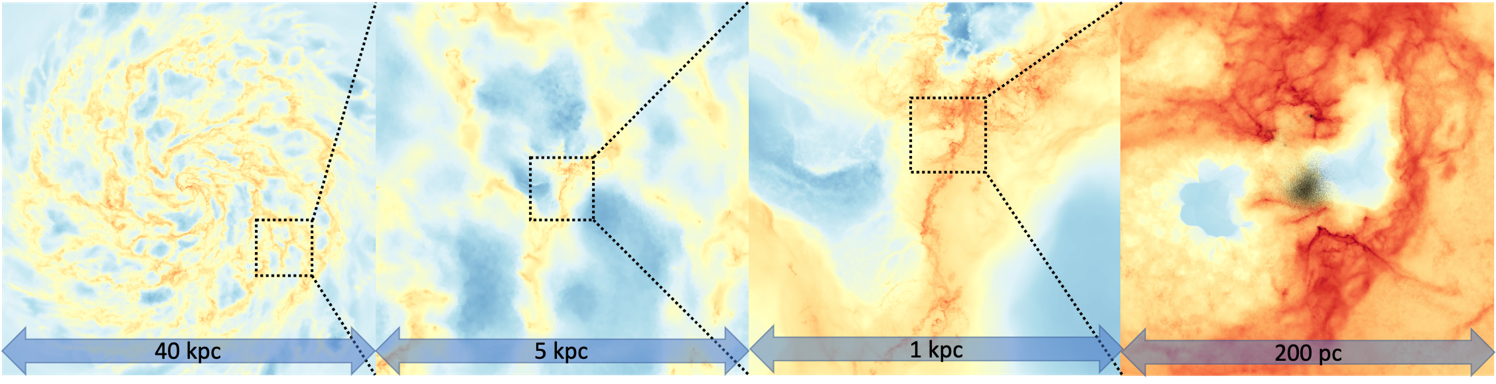
\includegraphics[width=\linewidth]{Outlook_img/Hui_sim.png}
    \caption{Gas surface density of a sequential zoom through a Milky Way-sized galaxy simulated using the moving-mesh code \texttt{Arepo}. The panels show: (1) a 40\,kpc face-on galactic disk; (2) a 5\,kpc local spiral structure; (3) one selected kpc-wide hyper-refinement region; and (4) a massive star-forming region centered at a star cluster (black dots). Credit: Hui Li.}
    \label{fig:hui-sim}
\end{figure}

\subsection{Applying machine-learning turbulence diagnostics beyond plasma simulations}
\fullsubsectionlabel{sec:awesom-beyond-plasma}

\begin{figure}[ht!]
    \centering
    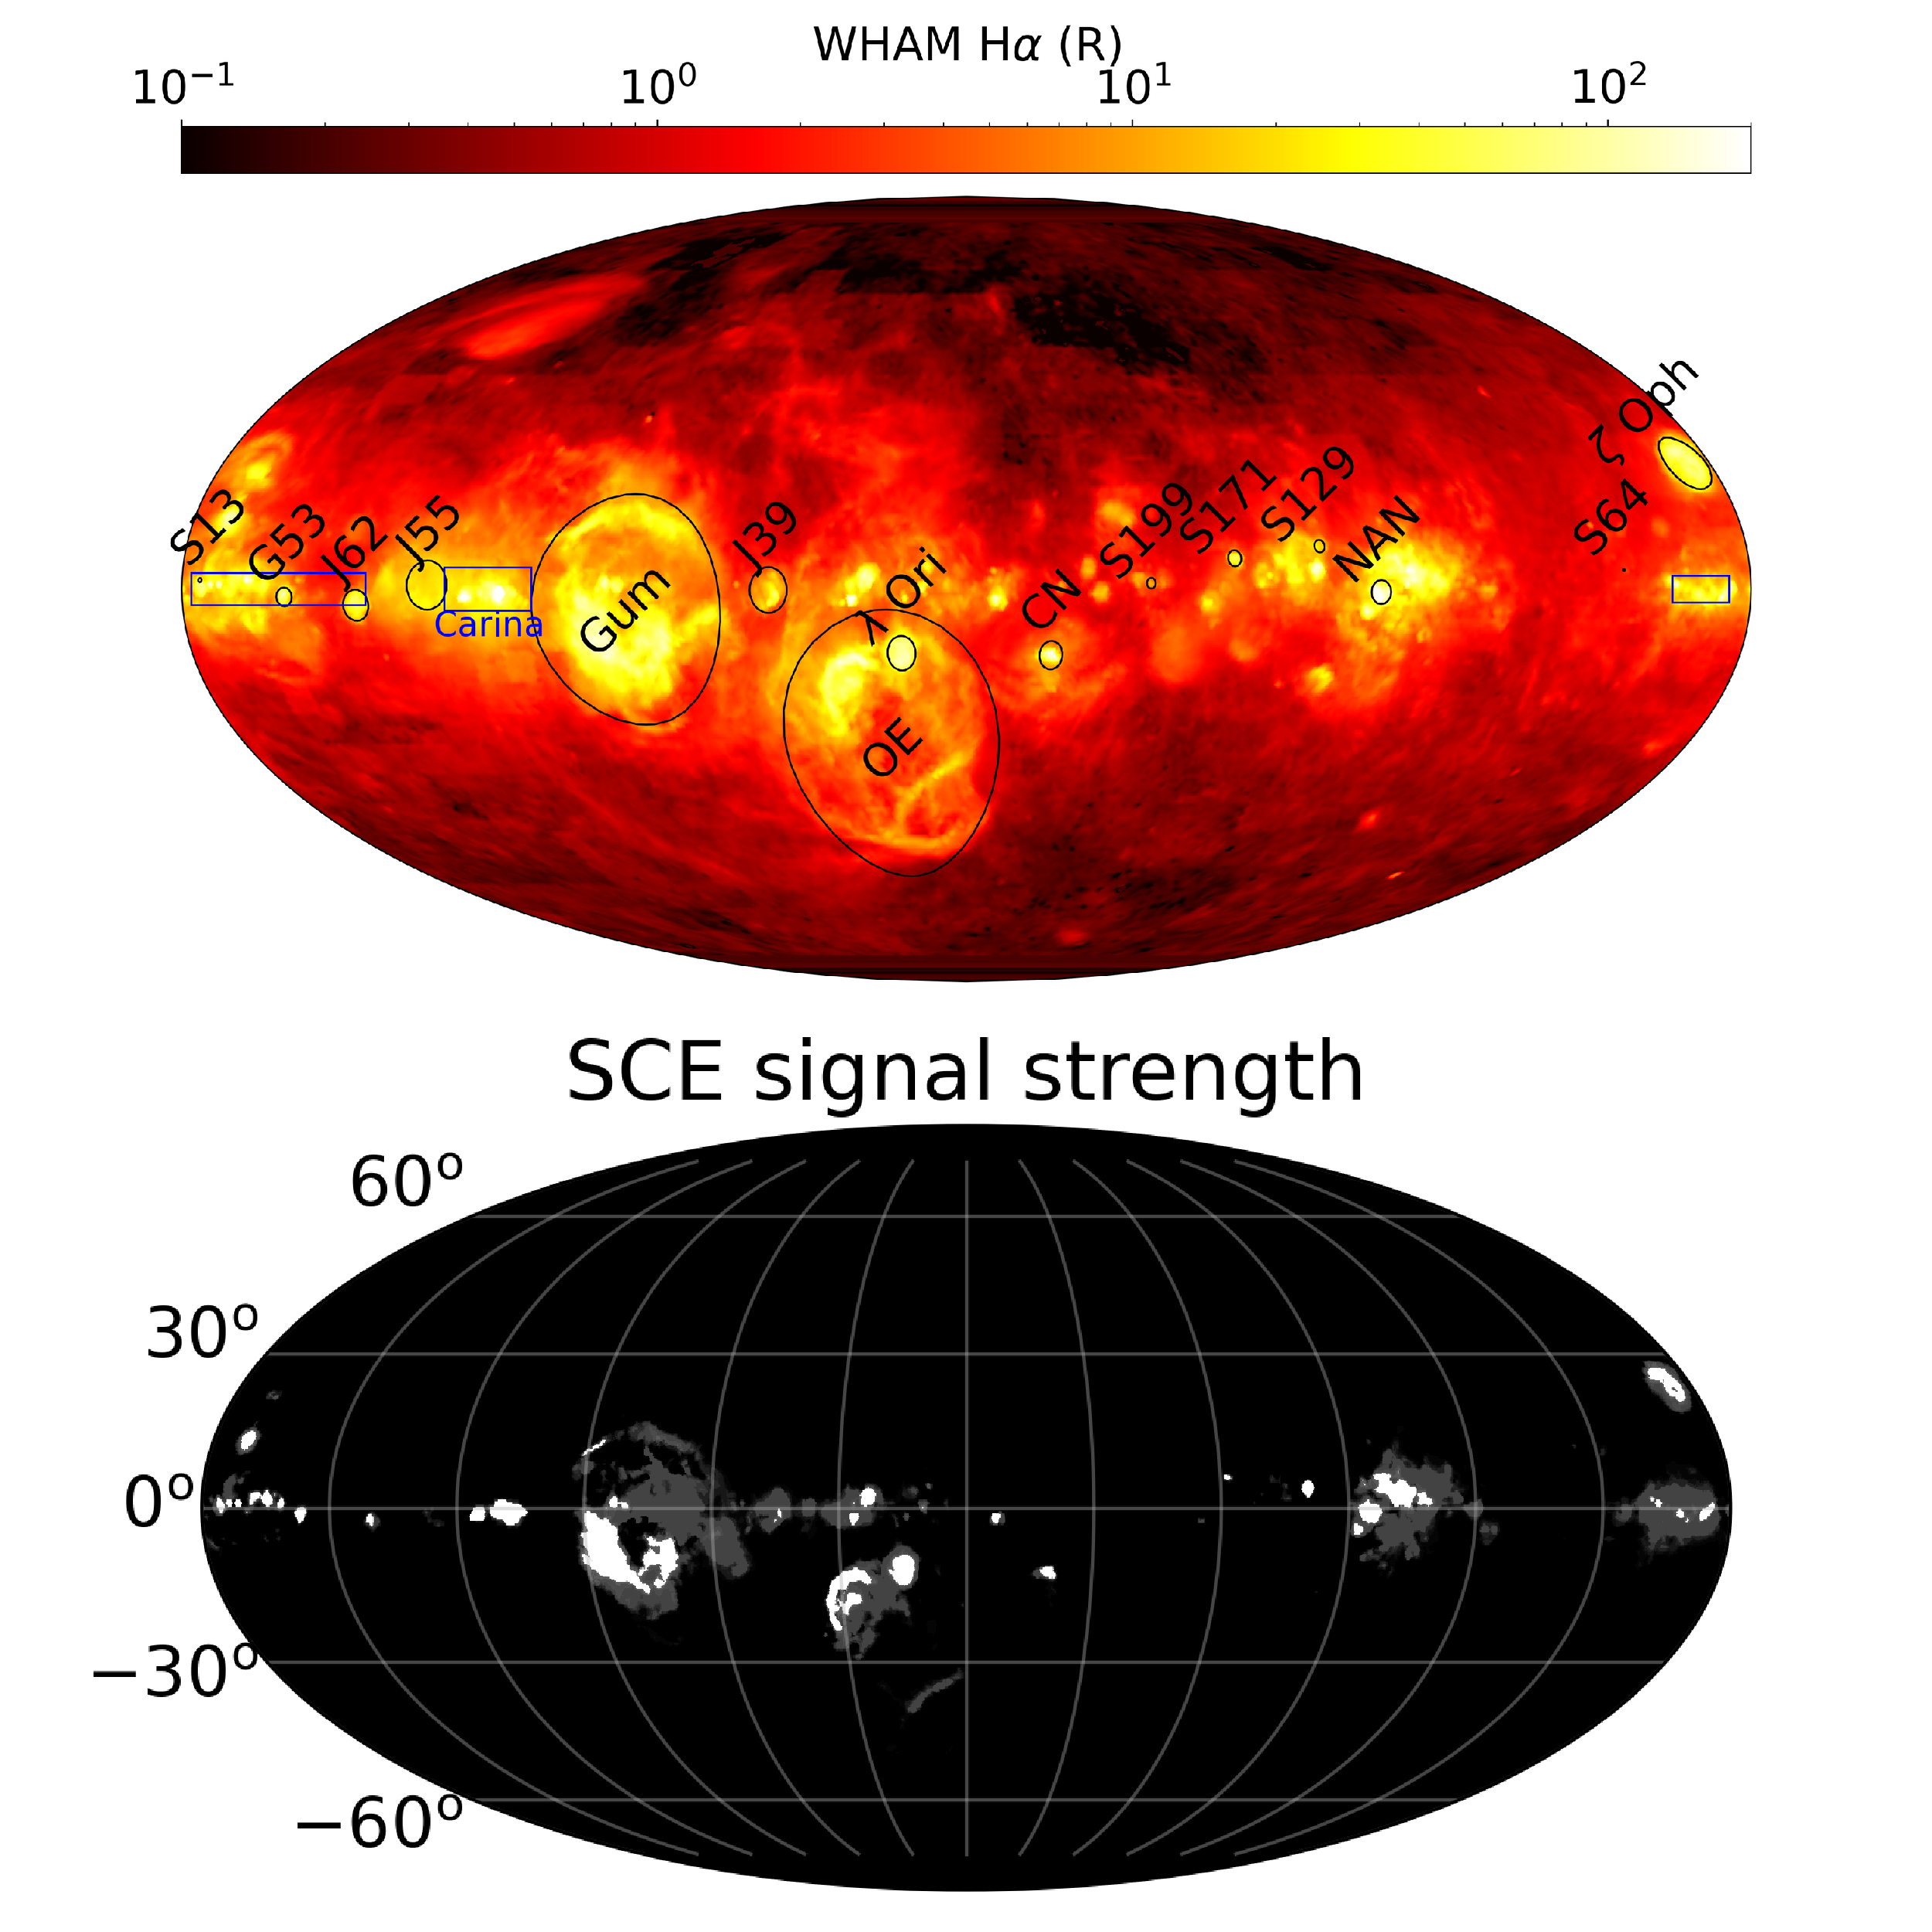
\includegraphics[width=\linewidth]{Outlook_img/SOM_Halpha.pdf}
    \caption{Preliminary application of \awesom\ to the all-sky Wisconsin H-Alpha Mapper (WHAM) \halpha\ survey \citep{haffner_wisconsin_2003}. Top: integrated \halpha\ intensity as a function of Galactic longitude and latitude, adapted from \citet{mccallum_halpha_2025}. Bottom: SCE signal strength obtained by combining multiple \awesom\ clustering realizations of the corresponding \halpha\ LOS velocity map. Regions of high SCE signal coincide with many star-forming regions and other prominent ionized structures, showing that the same unsupervised framework used for plasma-turbulence segmentation can also highlight coherent structures in observational ISM data.}
    \label{fig:som-halpha}
\end{figure}

Although \awesom\ was developed for plasma-turbulence segmentation, it can also be used for clustering or identification problems beyond the plasma domain.
As a demonstration, the online documentation\footnote{\url{https://awesom.readthedocs.io/en/latest/notebooks/iris.html}} applies the package to the Iris dataset \citep[][]{fisher_iris_1936}, a well-known non-linear classification problem.

An immediate extension of \awesom\ in the astronomy domain would be to apply the same unsupervised classification framework to high-dimensional observational maps, where the relevant structures are no longer current sheets but coherent regions of the multiphase ISM\@.
As an example, Figure~\ref{fig:som-halpha} shows an application to the WHAM survey, in which regions of high SCE signal in the \halpha\ LOS velocity data coincide with many star-forming regions and other prominent ionized structures.
This type of analysis can provide a data-driven method to define coherent ISM structures, such as star-forming regions or \ion{H}{2} regions, complementing existing rule-based methods.


\subsection{Connecting M87 simulations to X-ray velocity spectra}

\begin{figure}[t!]
    \centering
    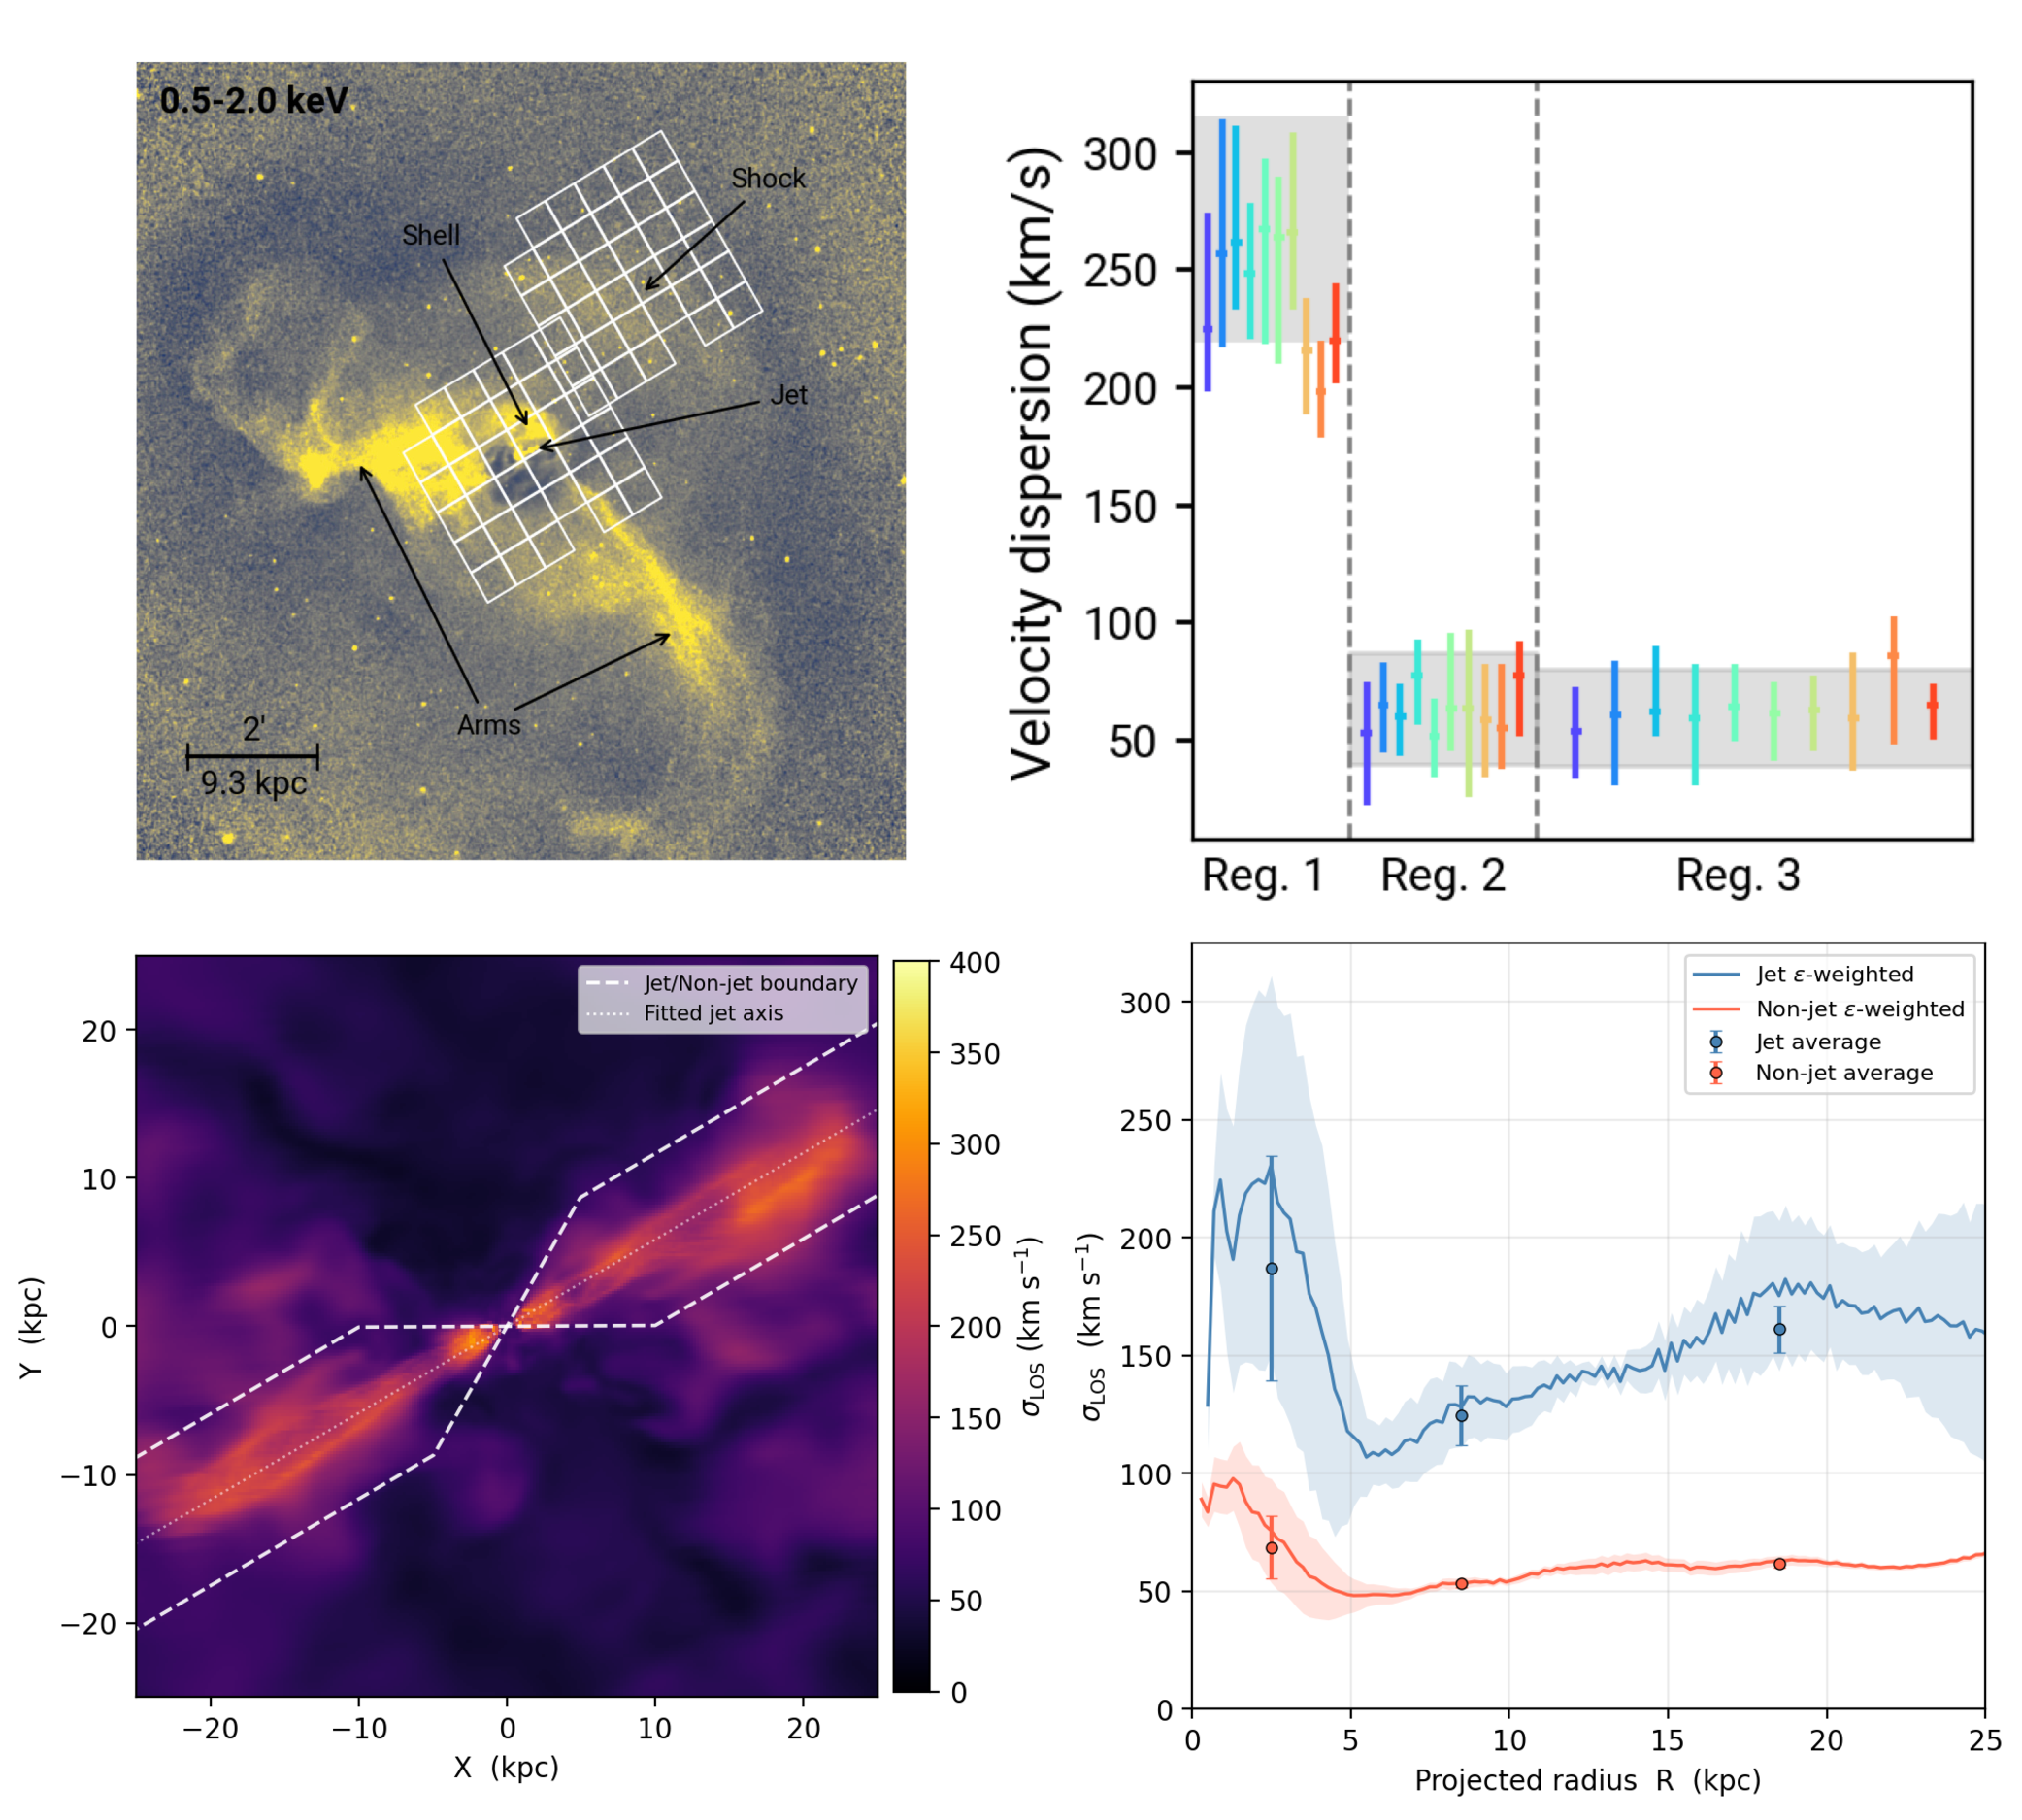
\includegraphics[width=\linewidth]{Outlook_img/Xray_los_sigma.pdf}
    \caption{Comparison between XRISM measurements of the M87 hot atmosphere and synthetic velocity dispersions from the simulations in Chapter~\ref{chap:sim}. Top left: \textit{Chandra} $0.5$--$2.0$\,keV image of the M87 core with the XRISM pointings overlaid, showing the jet, shell, shock front, and X-ray arms. Top right: XRISM (4.2 keV--7.0 keV band) LOS velocity dispersion in three projected radial regions, $0$--$5$\,kpc, $5$--$12$\,kpc, and $12$--$25$\,kpc. Images are adapted from \citet{xrism_collaboration_xrismresolve_2026}. Bottom left: simulated LOS velocity-dispersion map, with the dashed curves separating the jet and non-jet regions and the dotted line marking the projected jet axis. Bottom right: simulated radial profiles of the LOS velocity dispersion, $\sigma_{\rm LOS}$, in the jet and non-jet sectors, comparing unweighted and XRISM-band emissivity-weighted averages. This comparison makes the Chapter~\ref{chap:sim} simulation a direct benchmark against high-resolution observations in M87 \citep{ha_galaxy-_2026}.}
    \label{fig:xray-los-sigma}
\end{figure}

High-resolution X-ray spectroscopy now offers a direct observational benchmark for hot-gas velocity fields similar to those presented in Chapter~\ref{chap:sim}.
XRISM/Resolve recently measured LOS gas kinematics in the M87 atmosphere across three projected radial regions, finding a central velocity dispersion of $\sigma_{\rm LOS}=262^{+45}_{-38}\,\mathrm{km\,s^{-1}}$ within $0$--$5$\,kpc that then drops to $\sim 60\,\mathrm{km\,s^{-1}}$ from $5$--$25$\,kpc \citep{xrism_collaboration_xrismresolve_2026}.
This strong radial contrast highlights the central few kiloparsecs as the most turbulent region, where the AGN, jet, cavities, weak shocks, and X-ray shell coexist.
A direct comparison through mock observations also provides a more stringent target for simulations than density and temperature profiles alone, because the velocity dispersion directly constrains how mechanical energy is partitioned between coherent expansion, turbulent broadening, and bulk flows.

Figure~\ref{fig:xray-los-sigma} illustrates a preliminary comparison between the XRISM measurements and synthetic LOS velocity dispersions from the simulation in Chapter~\ref{chap:sim}.
The simulated maps show enhanced $\sigma_{\rm LOS}$ along the projected jet direction, while the non-jet regions are enhanced only in the central few kiloparsecs before plateauing at values similar to those measured by XRISM in the outskirts of the galaxy.
Further analysis with XRISM pointings along the jet and arms could test whether current jet prescriptions in galaxy simulations accurately model the kinetic-energy distribution of jet feedback.

\subsection{From meso-scale accretion to event-horizon GRMHD simulations}

One natural extension of Chapter~\ref{chap:sim} is to carry the meso-scale accretion flow all the way to the event horizon with GRMHD simulations.
Most horizon-scale simulations still initialize from ad hoc initial and boundary conditions, such as a torus of matter with an imposed poloidal or toroidal magnetic field.
Those setups have been useful for understanding generic black hole accretion, but they do not encode the multiphase morphology, angular momentum structure, or magnetic-field geometry produced by jet-driven turbulent mixing across galaxy-scale and meso-scale flows.
The next step in understanding multi-scale accretion in M87 is therefore to initialize event-horizon simulations directly from the gas distribution and magnetic-field geometry produced by meso-scale M87 simulations.

Such simulations would test how a realistic accretion morphology influences the flow around M87$^{\star}$, the launching of its jet, and the conditions required to build a magnetically arrested disk (MAD).
Adaptive mesh refinement can concentrate resolution near the disk and jet, allowing magnetic flux advection, jet power, and accretion variability to be followed in a setup that inherits structures from the larger-scale inflow.
The results enabled by these next-generation simulations would also create a more direct bridge to EHT observations: synthetic 230 GHz images and polarization maps from these simulations could be compared against existing M87$^{\star}$ observations and future time-dependent reconstructions of the black hole shadow.

The meso-scale simulations in Chapter~\ref{chap:sim} also show a warped accretion disk, with the angular momentum vector changing gradually with radius (see Figure~\ref{fig:main}).
If this warped disk is misaligned with the SMBH spin, Lense--Thirring precession should alter the inner disk orientation and may influence the direction of jet launching.
Future GRMHD simulations initialized from such warped inflows could therefore connect the angular momentum structure of the accreting gas to possible jet precession in M87, and test whether successive rings of misaligned gas can drive time-dependent changes in the jet nozzle direction.
In this way, the multi-scale approach developed in this dissertation can be extended from a model of black hole feeding to a model of the observable horizon-scale disk-jet system.

\begin{figure}[ht!]
    \centering
    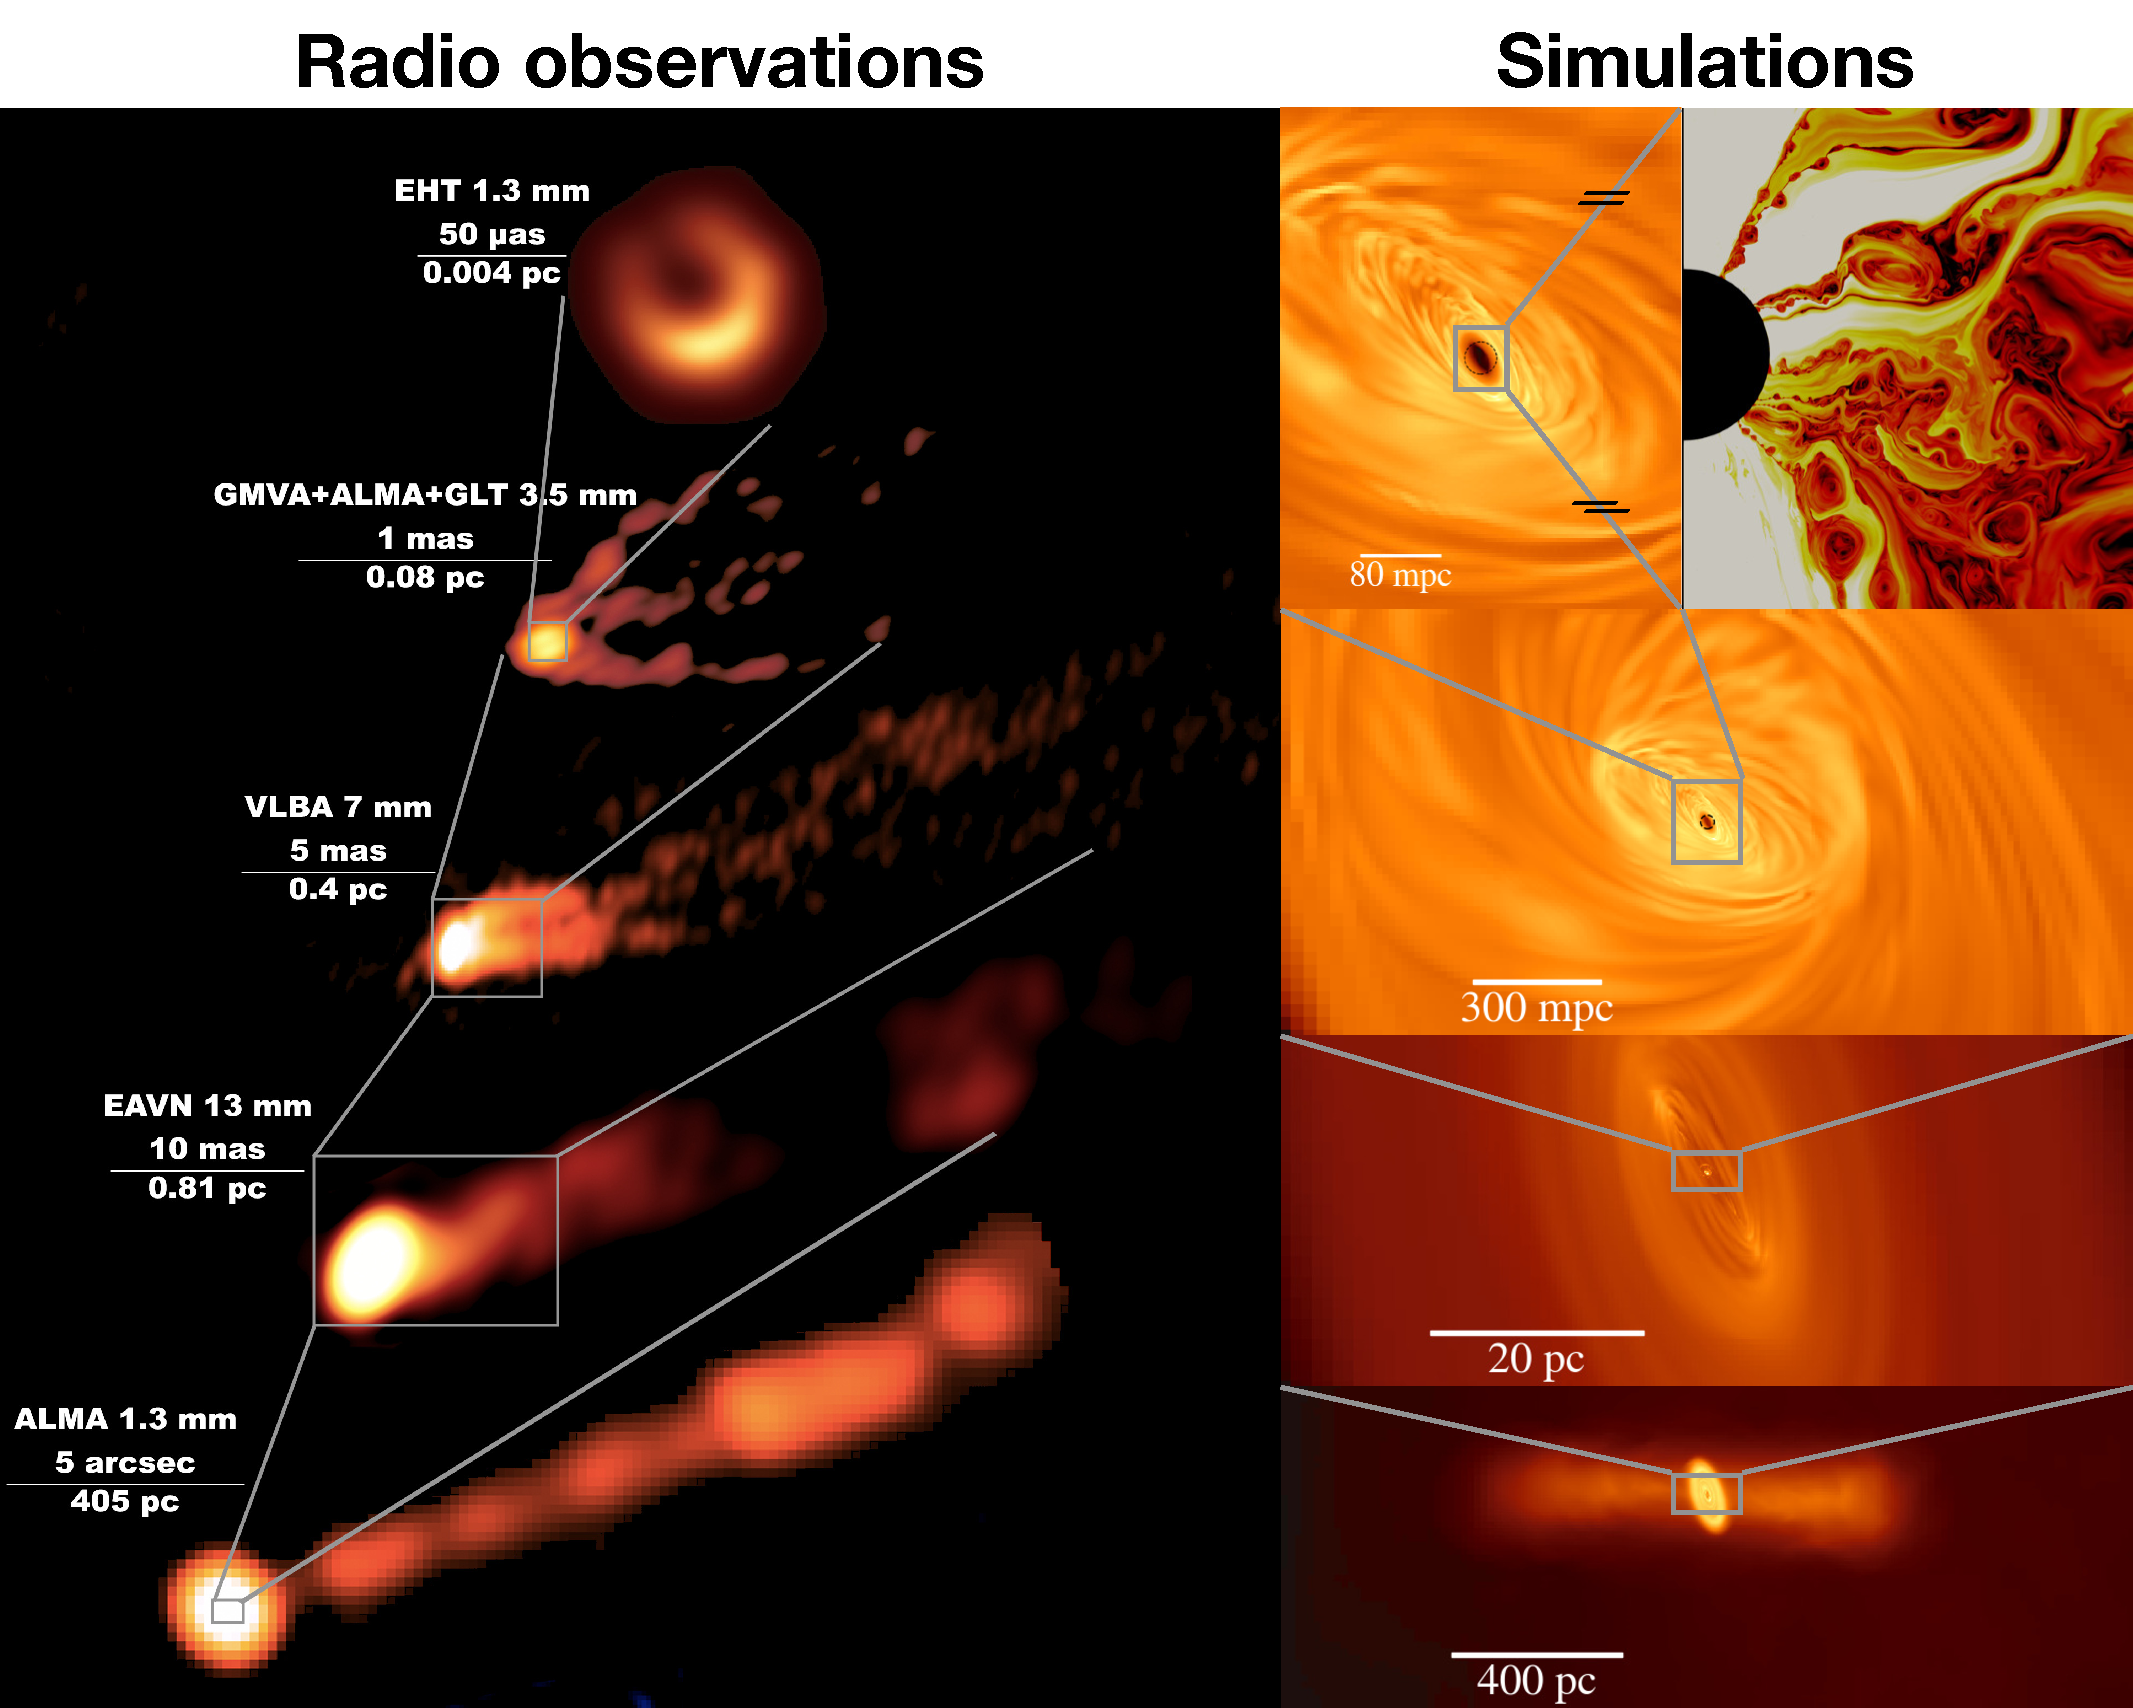
\includegraphics[width=\linewidth]{Outlook_img/obs-theory.pdf}
    \caption{The current state of modern observations and simulations in connecting a SMBH to its host galaxy. Left: observations of M87$^{\star}$, which resolve both the disk and the jet emission, adapted from \citet{algaba_broadband_2024}. Right: density projection plots from the multi-scale simulation presented in Chapter~\ref{chap:sim} \citep{ha_galaxy-_2026}. Window sizes range from $2$\,kpc to $0.5\,\mathrm{pc} \approx 10^3\,r_{\rm g}$ (gravitational radius). To understand the accretion process and multimessenger signals at the event-horizon scale (represented in the top right by a simulation of black hole accretion \citep{ripperda_magnetic_2020}), future GRMHD simulations can use initial conditions from this meso-scale accretion model.}
    \label{fig:main}
\end{figure}

\subsection{Reconnection, flares, and multimessenger signals}

The same event-horizon-scale simulations proposed in the previous subsection would also provide a path toward studying the high-energy signals produced by magnetic reconnection.
Bright TeV flares have been observed from M87 on timescales of several days, releasing a non-negligible fraction of the jet power during these events.
High-resolution GRMHD simulations suggest that these flares can be powered by reconnecting current sheets at several gravitational radii from the black hole, although the reconnection rate in ideal GRMHD simulations is often too slow to reproduce the observed variability \citep[e.g.,][]{ripperda_black_2022}.
Future work should therefore test whether more realistic accretion morphology, inherited magnetic-field structure, and effective resistivity prescriptions can reproduce reconnection-powered flares with both the correct energy spectra and timescales.

Another key challenge in accretion modeling is that magnetic reconnection events are still commonly identified and analyzed by hand.
This is manageable for a single prominent current sheet, but it becomes subjective and impractical when many reconnecting structures exist concurrently in a turbulent accretion flow.
The machine-learning framework developed in Chapter~\ref{chap:ml} provides a solution to make this measurement systematic: \awesom\ can be trained to identify reconnecting regions in GRMHD or PIC datasets, after which the spatial extent of each sheet can be used to measure inflow velocities, reconnection rates, and thermal dissipation profiles.
This would significantly accelerate efforts to understand current-sheet formation and energy dissipation through reconnection.

The same \awesom-based workflow also promises to enable modeling of reconnection-driven hadronic acceleration.
The source of ultra-high-energy cosmic rays (UHECRs) remains uncertain more than a century after their first detection, and recent IceCube observations of high-energy neutrinos from NGC 1068 have strengthened the case for particle acceleration in AGN environments \citep{collaboration_evidence_2022}.
In the corona region of AGNs, charged particles can meander between the two sides of a relativistic reconnection layer and gain energy during each crossing; similar acceleration may also occur in magnetically dominated turbulent regions near the equatorial current sheet, in flux tubes ejected during the MAD state, or along the jet boundary.
In future GRMHD simulations, test particles can be injected into the \awesom-identified reconnection layers to be followed through their acceleration and eventual escape from the simulation domain.
The energy spectrum of these particles would test whether low-luminosity AGNs such as M87$^{\star}$ can accelerate UHECR particles that later produce observable multimessenger signals.

A further extension of this analysis would integrate \awesom\ directly into GRMHD simulations as a runtime detector for reconnection events.
When the detector identifies a reconnecting layer, test particles could be injected at the site and followed until they leave the domain.
This approach would reduce the number of particles tracked throughout the full simulation and would also reduce the need to store dense restart outputs for post-processing.
The resulting particle spectra could then test whether the accretion flow around M87$^{\star}$ can produce UHECRs or high-energy neutrinos.

\section{Concluding Remarks}

Stellar kinematic surveys, kinetic plasma simulations, X-ray spectroscopy, and event-horizon modeling now constrain turbulence across physical scales from molecular clouds to black hole accretion flows.
Across these regimes, turbulence is becoming less an obscure signal inferred indirectly and more a measurable, well-constrained physical process that regulates star formation, plasma heating, black hole feeding, and feedback.
This dissertation has developed three complementary routes for constraining astrophysical turbulence: stellar velocity statistics for measuring turbulence in molecular clouds, machine-learning methods for identifying intermittent structures in relativistic plasma, and multi-scale simulations for connecting SMBH feeding to jet feedback in M87.
